\section{Design and use cases}

Practical usage of large language models can be broadly divided into two main scenarios: inference and parameter-efficient adaptation to downstream tasks. In this section, we outline the design of \textsc{Petals}, showing how it handles both scenarios and also allows easily sharing trained adapters between the users of the system.

\subsection{Inference of billion-scale models}\label{sect:design_inference}

When generating tokens, a client stores the model's token embeddings (which typically comprise a small fraction of the total parameter count and can fit in RAM in most modern laptops, servers, and workstations) locally and relies on servers to run Transformer blocks. Each server holds several \textit{consecutive} blocks, the number of which depends on the server's available GPU memory.
Before each inference session, the client finds a chain of servers that collectively hold all model layers.

Once the chain is formed, the client uses the local embedding layer to look up embedding vectors for prefix tokens, then sends those vectors to servers and receives new representations. Once the client obtains the outputs of the final block, it computes next token probabilities and repeats this process.
%\footnote{Most LLMs, including BLOOM, reuse the embedding matrix to compute next token probabilities}

While the session is active, servers store attention keys and values from past client inputs and use them for subsequent inference steps. Clients also store past inputs to each server so that if any server fails or goes offline, another one can quickly take its place. The procedure for finding servers and recovering from failures is detailed in Section~\ref{sect:networking}.

\paragraph{Client-side API.} To generate tokens with \textsc{Petals}, one first creates an \textit{inference session}. An inference session iteratively takes inputs as PyTorch tensors, runs them through all Transformer blocks and returns final representations as PyTorch tensors. Under the hood, sessions form server chains, hold cache, and recover from server failures in a way that is transparent to the user. An example of using an inference session is shown in Figure~\ref{fig:infernce_snippet}.

% Optionally, clients can send the same embeddings to multiple servers holding the same block. This allows client to verify the correctness of their inference by cross-checking clients. This can also be used to achieve consistently low latency if some servers experience delays.

\begin{figure}[tb]
\small
\begin{pythoncode}
# Initialize distributed BLOOM model
model = DistributedBloomForCausalLM \
    .from_pretrained("bigscience/bloom-petals")
input_ids = tokenizer(prefix_text)

with model.inference_session() as session:
    # Session maintains a set of servers that
    # store attention KV from previous steps
    for _ in range(sequence_length):
        # Compute the word embeddings locally
        hid = model.word_embeddings(input_ids)
        # Run distributed Transformer blocks,
        # store attention KV for future steps
        hid = session.step(hid)
        # Sample the next token locally
        probs = model.lm_head(hid)
        input_ids = sample_next_token(probs)
\end{pythoncode}
    \vspace{-5pt}
    \caption{A basic PyTorch code snippet for generation with a distributed BLOOM-176B model.}
    \label{fig:infernce_snippet}
    \vspace{-10pt}
\end{figure}

\paragraph{System requirements.} For BLOOM-176B inference, clients need at least 12 GB RAM, most of which is used to store 3.6B embedding parameters. We recommend at least 25 Mbit/s bidirectional bandwidth to avoid bottlenecks in network transfers. Simple greedy inference can use any CPU that runs PyTorch, but more advanced algorithms (e.g., beam search) may require a GPU.

In turn, servers need at least 16 GB of CPU RAM, 100 Mbit/s bandwidth and a GPU with at least 8~GB of memory.

\paragraph{Chat application.} We also provide an example application that lets users chat with LLMs in a messenger-like user interface (see Figure~\ref{fig:chat_app}). The application supports BLOOM-176B and BLOOMZ-176B, a version of BLOOM fine-tuned to better perform in the zero-shot regime~\cite{bloomz}. The application is comprised of the \textit{frontend} and the \textit{backend}.
The frontend is a web page that allows users to communicate with the model by prompting it with text and receiving the generated output.
The backend is a Flask web server that uses the \textsc{Petals} client to run inference over the swarm. It accepts requests via HTTP or Websocket protocols, so anyone can develop their own applications using our backend for inference.

%figure moved to the other column

\subsection{Training for downstream tasks}\label{sect:design_training}

While LLMs achieve high quality on many problems with simple prompt engineering~\citep{gpt3}, they often need training to achieve the best results. Traditionally, this is done by fine-tuning all model parameters on the downstream task.
%Adapting a single large pre-trained language model to multiple tasks and domains is a de facto standard for many downstream generation and natural language understanding (NLU) applications. \textit{Full fine-tuning}, which updates all model parameters, often demonstrates state-of-the-art performance.
However, for very large models, this strategy becomes impractical due to hardware requirements. For example, fine-tuning BLOOM-176B with Adam would require almost 3~TB of GPU memory to store model, gradients, and optimizer states.

To combat this issue, the NLP community has developed \textit{parameter-efficient fine-tuning} methods that keep most of the pretrained model intact. Some of them~\citep{sung2021training,guo2021parameter} choose a subset of existing parameters, others~\citep{hu2021lora, houlsby2019parameter, ptune-liu, ptune-lester, ptune-v2, tfew} augment the model with extra trainable weights.

Despite their lower memory requirements, parameter-efficient approaches are often competitive with full model fine-tuning \citep{hu2021lora,ptune-v2,yong_adapting} and even outperform it in low-data regimes~\citep{2205.05638}. Another appealing property of these approaches for our use-case is that they allow rapidly switching a pretrained LLM between different uses.

%note: the paragraph below was commented due to spacing cosntraints
% -- It can be reintroduced later if we have some room to spare
% Overall, efficient adaptation of large language models is an essential direction that makes them appealing for real-world applications. Thus, in our demonstration, we put significant effort into providing \textbf{accessible}, \textbf{user-friendly}, \textbf{reliable} and \textbf{efficient} service for BLOOM-176B adaptation.

\begin{figure}[tb]
    \centering
    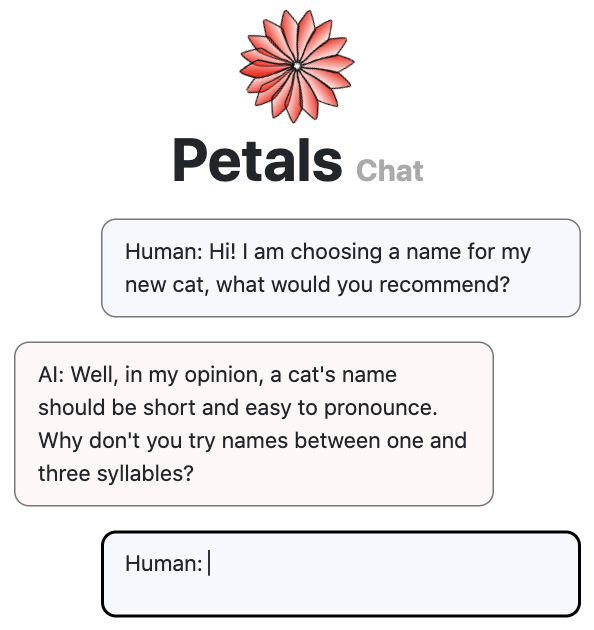
\includegraphics[width=0.9\linewidth]{resources/chat_app.png}
    % \vspace{-5pt}
    \caption{A chat application that runs BLOOM-176B or BLOOMZ-176B over the \textsc{Petals} swarm, available at \texttt{\href{https://chat.petals.ml}{https://chat.petals.ml}}}
    \label{fig:chat_app}
    \vspace{-10pt}
\end{figure}

\paragraph{Distributed fine-tuning.} The core principle of fine-tuning in a distributed network is that clients ``own'' trained parameters while servers host original pretrained layers. Servers can run backpropagation through their layers and return gradients with respect to activations, but they \textit{do not update the server-side parameters}. Thus, clients can simultaneously run different training tasks on the same set of servers without interfering with one another.

% \begin{figure}[tb]
%     \centering
%     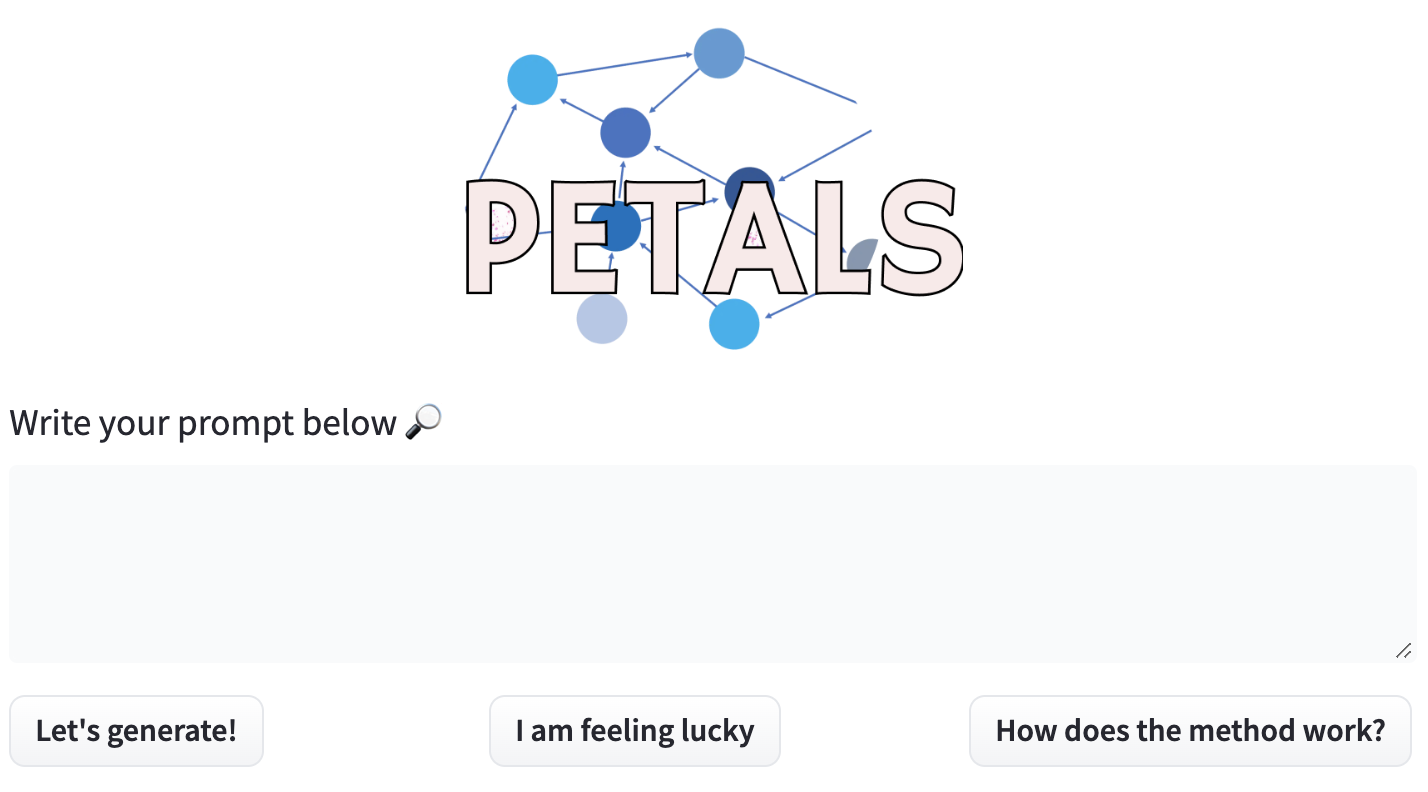
\includegraphics[width=0.7 \linewidth]{resources/GUI.png}
%     \caption{A prototype of the user interface for inference with \textsc{Petals}.}
%     \label{fig:infernce_ui}
%     \vspace{-5pt}
% \end{figure}

% In more detail, each user locally stores a few trainable parameters, e.g, tunable prompts or adapters. At each training iteration, a client sends his inputs and parameters to the remote model. A sequence of servers perform forward and backward operations and send the gradients w.r.t. client's parameters back. The client receives the gradients and locally updates the parameters. 

To illustrate this principle, we first review an example of soft prompt-tuning for text classification and then generalize it to other methods and tasks.
Similarly to Section~\ref{sect:design_inference}, clients store the embedding layers locally and rely on servers to compute the activations of Transformer blocks. In this fine-tuning scenario, a client needs to store trainable soft prompts (task-specific input embeddings) and a linear classification head. 

For each training batch, the client routes its data through a chain of remote servers to compute sentence representations, then obtains predictions with the classifier head and computes the cross-entropy loss.
%NOTE: this intentionally avoids talking about load balancing and fault tolerance
During backpropagation, the client runs its data through the same chain of servers in reverse order to compute gradients for the learned prompt vectors. Having obtained those gradients, the client can use a regular PyTorch optimizer to update the parameters of both the head and the prompts, then proceed to the next minibatch.

\paragraph{User interface.} To allow users greater flexibility in their training workloads, we made distributed backpropagation module compatible with the PyTorch Autograd engine. Like in the inference stage, this module handles fault tolerance and load balancing transparently to the user while allowing them to access intermediate activations and insert custom PyTorch modules. Figure~\ref{fig:training_snippet} shows an example training code snippet.

%provide state-of-the-art parameter-efficient fine-tuning methods, which do not update the initial model weights\citep{p-tune. p-tune-v2, lora}. 
This interface can also support other popular parameter-efficient fine-tuning algorithms, such as LoRA~\citep{hu2021lora} or prefix tuning~\citep{li-liang-2021-prefix}. Finally, users can insert custom local modules after some of the  existing blocks, which could allow use-cases like retrieval-augmented generation~\citep{retro,rag}.% or sparse Mixture-of-Experts layers~\citep{Lepikhin2020GShardSG,switch,base}.

\begin{figure}[tb]
\small
\begin{pythoncode}
# Use distributed BLOOM with soft prompts
model = AutoModelForSequenceClassification \
    .from_pretrained(
        "bigscience/bloom-petals",
        tuning_mode="ptune", pre_seq_len=5)
# Define optimizer for prompts and linear head
opt = torch.optim.AdamW(model.parameters())

for input_ids, labels in data_loader:
    # Forward pass with local & remote layers
    out = model.forward(input_ids)
    loss = cross_entropy(out.logits, labels)

    # Distributed backward w.r.t. local params
    loss.backward() # Compute prompts.grad
    opt.step() # Update local params only
    opt.zero_grad()
\end{pythoncode}
\vspace{-5pt}
\caption{A basic PyTorch code of soft prompt tuning for sequence classification with \textsc{Petals}.}
\label{fig:training_snippet}
\vspace{-10pt}
\end{figure}


% \textbf{System requirements.} The minimal training script for soft prompt-tuning requires 16GB RAM and benefits from high network bandwidth.
% Similarly to Section~\ref{sect:design_inference}, nearly half of all memory is used on pre-trained embeddings, while the few trainable parameters have negligible memory footprint. Intermediate activations also use little memory due to the use of gradient checkpointing~\citep{gradient_checkpointing_autograd,gradient_checkpointing_dl}. Naturally, workloads with more trainable parameters will require additional memory and often benefit from having a local GPU.


% This training procedure makes the system \textbf{cheap} and \textbf{accessible} since the users can perform the model adaptation on their laptops, desktops or Colab notebooks. The minimum hardware requirements are only <TODO> GBs of RAM and $100$ Mbps network speed.

% Moreover, since the adaptation methods do not update the parameters of the pre-trained model, multiple users can solve their individual tasks at the same time. In addition, researchers and developers can readily incorporate their custom PEFT methods.

% Importantly, all distributed details are hidden inside standard PyTorch methods. Thus, users only have to run a simple PyTorch training loop to adapt the BLOOM-176B to their tasks. We provide an example of the the training code in Figure~\ref{figure:training_snippet}. During the demonstration, users will be able to give it a try and solve sequence classification and <TODO: some generative task> on public datasets.

% \begin{itemize}
%     \item \textbf{Accessible:} Each user can adapt the model on his desktop / laptop / colab having only <TODO> GBs of RAM and $100$ Mbps network speed; 
%     \item \textbf{Flexible:} 
%         \begin{itemize}
%             \item Multiple users can solve their individual tasks independently at the same time;
%             \item Users can customize or incorporate their own adaptation methods;
%         \end{itemize}
%     \item \textbf{High-quality:} Suggest state-of-the-art parameter-efficient model adaptation methods;
%     \item \textbf{User-friendly:} High-level API for regular users and standard PyTorch training code for developers and researchers;
% \end{itemize}

% \textbf{Parameter-efficient fine-tuning.} Exists. Describe prompt-tuning, adapters, yield from 2205.05638. Cite relevant papers.

% Users can hold their prompts / adapters locally with limited RAM. Two users can simultaneously train two prompts / adapters without interfering with one another. Servers only hold ``permanent'' bits of the model.

% \textbf{Demo part with prompt tuning:} explain what we provide. Client stores only embeddings and learned prompts -> prompt-tuning can be done in colab / on a commodity desktop. Code is similar to training locally.


% \textbf{Flexible interface for researchers.} Explain how researchers can insert their own custom modules for RAG / RETRO / MoE / PKM in the middle of the model. Supports torch autograd.



% FILLER TEXT TO ACCOUNT FOR MISSING CONTENT \lipsum[5]


\subsection{Sharing and reusing trained modules}
\label{sect:design_ecosystem}

Although most fine-tuned extensions for pretrained models can be easily shared as-is, simplifying the workflow for sharing these extensions enables users to more easily adapt the model to their target scenario. Indeed, existing model hubs~\citep{wolf-etal-2020-transformers, tfhub, torchhub} have gained immense popularity due to many supported models and ease of use, especially when vetting different pretrained models for a given problem. One particularly relevant project is AdapterHub~\citep{adapterhub}, a repository of trained adapters accompanied by a library with implementations of different adaptation methods. While \textsc{Petals} does not depend on AdapterHub, it is possible to leverage this library for training adapters in the distributed setting.
%We were also inspired by it when designing our streamlined solution for adapter sharing.
Instead, we support sharing modules trained by users via the Hugging Face Hub (also used as a backend by AdapterHub). Its infrastructure and the corresponding open source library simplify the learning process for users already familiar with the ecosystem. Because the primary navigation mechanism on the Hugging Face Hub are tags that have been applied to uploaded modules, a user only needs to the task it was trained on and the model upon which the adapter was built. Uploading the weights and the code of the fine-tuned module is done by committing them to a Git repository.
When navigating the Hub, users can choose the most suitable adapters by filtering the list of all available modules by the required tags.